% for ACM papers
\documentclass[sigconf, anonymous]{acmart}
% for IEEE papers
%\documentclass[conference,compsoc]{IEEEtran}

% \usepackage{amsmath,amssymb,amsfonts}
\usepackage{graphicx}
\usepackage[linesnumbered,lined,vlined,ruled,commentsnumbered,noend]{algorithm2e}
\usepackage{textcomp}
\usepackage{xcolor}
\usepackage{listings}
\usepackage{url}
\usepackage{xspace}
\usepackage{multirow}
\usepackage{balance}
\usepackage{ctable}
\usepackage{listings}
\usepackage{color}
\usepackage{graphicx}
\usepackage{subcaption}
\usepackage[nobiblatex]{xurl}

\usepackage{multirow}
% \usepackage{algorithmic}

\usepackage{algpseudocode}
\usepackage{caption}
\usepackage{subcaption}

\usepackage{cleveref}
\usepackage{acronym}
\usepackage{fancybox}
\usepackage{verbatim}
\usepackage[normalem]{ulem}
\usepackage{float}
\usepackage{newfloat}
\usepackage{mdframed}
\usepackage{enumitem}
\usepackage{booktabs}
\usepackage{pifont}

% Useful macros for paper writing

\definecolor{red}{RGB}{255,0,0}
\definecolor{green}{RGB}{18,220,168}

\newcommand{\ie}{i.e.,\xspace}
\newcommand{\eg}{e.g.,\xspace}
\newcommand{\etc}{etc.\xspace}
\newcommand{\etal}{\textit{et al.}\xspace}

\newcommand{\mypar}[1]{\vspace*{0.5ex}\textbf{#1}}
\newcommand{\mypari}[1]{\vspace*{0.5ex}\emph{#1}}
\newcommand{\company}{anonymous company\xspace}%

\newcommand{\cmark}{\ding{51}}%
\newcommand{\xmark}{\ding{55}}%
%color options: white, black, red, green, blue, cyan, magenta, yellow
\newcommand{\blank}[1]{\textcolor{red}{(#1)}}
\newcommand{\explain}[1]{\textcolor{blue}{(#1)}}

\newcommand{\dingli}[1]{\textcolor{red}{(DL: #1)}}
\newcommand{\xiao}[1]{\textcolor{blue}{(XIAO: #1)}}
\newcommand{\shaofei}[1]{\textcolor{green}{(LI: #1)}}
%\newcommand{\jp}[1]{\texttt{(JP: #1)}}

\renewcommand{\algorithmicrequire}{\textbf{Input:}}  % Use Input in the format of Algorithm
\renewcommand{\algorithmicensure}{\textbf{Output:}} % Use Output in the format of Algorithm

\newcommand{\INPUT}{\item[\algorithmicinput]}
\newcommand{\OUTPUT}{\item[\algorithmicoutput]} 
\newcommand{\name}[1]{\textit{#1}}
\newcommand{\mname}[1]{\mathit{#1}}
\newcommand{\func}[1]{\texttt{#1}}
\newcommand{\toolname}{\textsc{NodLink}\xspace}
\newcommand{\toolnameu}{\textsc{Unicorn}\xspace}
\newcommand{\toolnameh}{\textsc{Holmes}\xspace}
\newcommand{\cadets}{\textsc{Cadets}\xspace}
\newcommand{\theia}{\textsc{Theia}\xspace}
\newcommand{\trace}{\textsc{Trace}\xspace}
\newcommand{\avedis}{two\xspace}
\newcommand{\insightone}{Attack Affinity\xspace}
\newcommand{\insighttwo}{Anomaly Polymerism\xspace}
\newcommand{\anosec}{AnonymousSec\xspace}
\newcommand{\activityanom}{Activity level Anomalies\xspace}
\newcommand{\eat}[1]{}
\acrodef{wp}[WP]{Website Fingerprinting}
\acrodef{apt}[APT]{Advanced Persistent Threats}
\acrodef{lol}[LotL]{Living-Off-The-Land}
\acrodef{ids}[IDS]{Intrusion Detection System}
\acrodef{vae}[VAE]{Variational AutoEncoder}
\acrodef{re}[RE]{reconstruction error}
\acrodef{sv}[SV]{Stableness Value}
\acrodef{as}[AS]{anomaly score}
\acrodef{gas}[GAS]{graph anomaly score}
\acrodef{etw}[ETW]{Event Tracing for Windows}
\acrodef{e3}[E3]{Engagement 3}
\acrodef{e5}[E5]{Engagement 5}
\acrodef{ttp}[TTPs]{Tactics, Techniques, and Procedures}
\acrodef{hsg}[HSG]{High-level Scenario Graph}
\acrodef{nlp}[NLP]{Natural Language Processing}
\acrodef{dg}[DG]{Detection Graph}
\acrodef{poi}[POI]{Point of Interest}
\acrodef{iv}[IV]{Important Value}
\acrodef{sg}[SG]{Suspicious Graph}
\acrodef{mttd}[MTTD]{Mean Time to Detect}
\acrodef{soc}[SOC]{Security Operations Center}
%stuff for listings package

%\newfloat{program}{h}{eqn}
%\DeclareFloatingEnvironment[]{component}
\newlength{\MaxSizeOfLineNumbers}%
\settowidth{\MaxSizeOfLineNumbers}{99}% Adjust to maximum number of lines
\addtolength{\MaxSizeOfLineNumbers}{.5ex}%
\definecolor{keywordcolor}{rgb}{0.8,0.1,0.5}
\definecolor{lightlightgray}{gray}{.96}
\definecolor{lightgray}{gray}{.925}
\definecolor{medlightgray}{gray}{0.7}
\definecolor{medgray}{gray}{0.4}
\definecolor{darkgray}{gray}{0.35}
\definecolor{nearblack}{gray}{0.15}

\lstset{%
language={Java}, 
columns=fullflexible, 
basicstyle=\color{nearblack}\scriptsize,
numbers=left,
identifierstyle=\color{black},
keywordstyle=\color{keywordcolor}\bfseries,
commentstyle=\color{medgray}\itshape,
stringstyle=\color{blue}\ttfamily\scriptsize,
showspaces=false,
showstringspaces=false,
showtabs=false,
tabsize=2,
emphstyle=\color{black}\gbox,
breaklines=true,
numbersep=4pt,
xleftmargin=\MaxSizeOfLineNumbers,
xrightmargin=0.5em,
framexleftmargin=1em,
firstnumber=auto,
showlines=true,
frame=none,
string=[b]",
escapechar=@
}%


%stuff for cleveref
%\crefname{figure}{Figure}{Figures}
\crefname{component}{Component}{Components}
%\crefname{algocf}{Algorithm}{Algorithms}
%\crefname{algorithmic}{Algorithm}{Algorithms}


\begin{document}
\title{A Template for Technical Papers} 
%for IEEE papers
%\maketitle
\begin{abstract}
    This is a template project for writing technical papers for system/security/SE papers. If you are writing a paper about a new technique, you may first try to fill the blanks in the paper for the first draft and then polish the language later. Before you write the paper, please first make clear the topic sentence of your paper by filling blanks in the next paragraph. 

    By introducing a novel, non-trivial, reasonable strategy \blank{}, we address a challenging technical problem \blank{} that existing techniques have not well addressed. Therefore, we can better satisfy an important technical requirement \blank{}. 

    \blank{} are slots that you need to fill. In your first draft, please keep the brackets and directly put your answers in the blank. Then, people can quickly track your answers and tell you which part should be strengthened. 

    \explain{} are some comments and explanations that helps you to understand to blanks.
\end{abstract}
%for ACM papers
\maketitle

\section{Introduction}


The technique requirement \blank{} is important for \blank{} reasons. \explain{These are a few possible ways to prove the requirement is important. Below are a few examples.} First, \blank{governments or big companies say it is important~\cite{}\cite{}\cite{}\cite{}}. Second, \blank{Big companies invest a lot of money in the requirement. The market worthes XXX billion dollars~\cite{}\cite{}\cite{}\cite{}}. Third, \blank{A lot of previous papers say this is an important requirement~\cite{}\cite{}\cite{}\cite{}}. Fourthm \blank{A lot of techniques are built upon this requirement~\cite{}\cite{}\cite{}\cite{} }.

There are \blank{} types of solutions that aims to meet the requirement \blank{}, but the cannot satisify the requirement well. The first type is \blank{}, it cannot well satisify the requirement due to the limitation \blank{}. The second type is \blank{}, it cannot well satisify the requirement due to the limitation \blank{}.
The second type is \blank{}, it cannot well satisify the requirement because \blank{}. \explain{more if needed, add references if needed}

Existing techniques cannot well satisfy the requirement because they fail to address a technical problem \blank{}, which is important to the requirement for \blank{} reasons. First,\blank{}. Second, \blank{}. Third, \blank{}. \explain{Sometimes the reasons are abvious, then you may not list the reasons explicitly and you can merge this paragraph to the previous one}.  

Addressing the technical problem is challenging  because of \blank{term 1}, \blank{term 2}, and \blank{term 3}. \explain{summarize the challenging with a few terms/words}. Specifically, the technical problem is difficult because of \blank{} reasons. 
\explain{These are a few examples.} First, \blank{Term 1 is diffucult because it requires solving an NP-hard problem XXX. Existing solutions to XXX can only provide an approximation. For example, A solves XXX with a B technique, that over/under-approximate the result. For our problem, it is particularly challenging to balance the accuracy and run-time overhead. } Second,  \blank{Term 2 is difficult because it requires a lot of engineering effort. For example, we need to reverse engineer a large binary code. Unfortunately, the document of the binary is not available/clear. We need to analyze the assemblly manualy.  } Third, \blank{Term 3 is difficult because there are constraints on energy/overhead/time-limit. In practice, the technique requirement is about mobile/IoT/Cloud environments that have strict constraints on energy/money. Existing techniques, such as XXX and XXX, cannot address term 3 because they cannot meet the requirements of energy/money. } Fourth, \blank{Term 3 is difficult because there is a conflict between A and B. On the one hand, satisfying A is important because of X. On the other hand, satisfying A is important because of Y. How to balance A and B is very difficult. }

In this paper, we propose a novel strategy \blank{} that addresses the technical problem \blank{} for the first time. Our strategy consists of \blank{} steps. First, \blank{}. Second, \blank{}. Third, \blank{}.


Our strategy is reasonable because it is motivated by \blank{} valid insights/observations. \explain{These are a few examples.} The first insight is \blank{}. It is valid because \blank{paper A, B, and C have reported it.}  The second insight is \blank{}. It is valid because \blank{we provide experiment to support it.} The third insight is \blank{}. It is valid because \blank{we have a solid reasoning about it.} The fourth insight is \blank{}. It is valid because \blank{we can provide a mathmatical proof.} 


Our strategy is novel for \blank{} reasons. First,\blank{we are the first who find the insights}. Second, \blank{insight 1 is old, but we are the first who apply it to the technical problem. Then we made necessary non-trivial adjustments to it}. Third, \blank{we are the first ones that provide the reasoning about the insights}. 


Our strategy is non-trivial because it encounters \blank{} technical/engineering challenges. \explain{These are a few examples.} First, \blank{the data volume is high. We need to efficiently process the data}. Although there are \blank{a few related solutions, such as A and B,}, they cannot be used to solve our problem easily because \blank{}. We handle this challenge by \blank{using a novel cache strategy that keeps hot data in memory.} Second, \blank{there is not unified data format.} Although there are \blank{a few related solutions, such as A and B,}, they cannot be used to solve our problem easily because \blank{}. We address this challenge by  \blank{using a novel NLP model that automatically embeds words into vectors. Our model is particularly efficient for our problem because of A}. Third, \blank{we do not have enough labels in the training dataset}. Although there are \blank{a few related solutions, such as A and B,}, they cannot be used to solve our problem easily because \blank{}. To address this challenge, we uses \blank{a novel semi-supervised model that automatically learns labels of unlabbeled data points. Our model is particularlly effetive for our problem becauseXXX}

We show our strategy satisfies the requirement better and addresses the technical problem with valid insights with a realistic experiment environment \blank{}. Our datasets are realistic because \blank{}. Our system configuration is realistic because \blank{}. 

To show that our strategy satisfies the technique requirement better with \blank{} aspects and compare them to \blank{} baselines. For the first aspect, we measure the metric \blank{}. Our strategy is \blank{X\%} better than the baselines. For the second aspect, we measure the metric \blank{}. Our strategy is \blank{X\%} better than the baselines.  For the second aspect, we measure the metric \blank{}. Our strategy is \blank{X\%} better than the baselines.  

To show our strategy addresses the technical problem, we measure metric \blank{}. This metric can prove that the technical problem is addressed because \blank{}. The result is \blank{}, which proves that the problem has been addressed. 

To show our strategy is reasonable, we measure the metric \blank{} to validate the insight \blank{}. The metric can prove the validity of the insight \blank{} because \blank{}. The result is \blank{}. 

\explain{Optional, sometimes you are not lucky enough to have this} We further validate the usefulness of our strategy in a production environment \blank{}. This environment is from \blank{}. Our strategy detects bugs/attacks/optimizes in commercial software or network environment. 

We summarize our contributions as follows \explain{Below are a few examples}:
\begin{itemize}
    \item We propose a novel strategy \blank{}.
    \item We propose find \blank{} new insghts, which are \blank{}
    \item We implement the strategy as a tool,\blank{}, and integrate it into a commercial enviroment. 
    \item We thoroughly evaluate our strategy with commercial dataset and real production environment. 
\end{itemize}
% Considering the disadvantages of the preceding works, we find that as for real-time model, we can neither consider the information of provenance data in great detail nor extract the provenance data to high-level. When considering the data in great detail, it will face an unacceptable computational overhead. When extracting to high-level, the detection will be too coarse-grained for analysts. Thus, it is promising to filter out redundant information with little computation overhead and conduct careful inspection on highly suspicious events or nodes. Then we can quickly reconstruct the attack scenario from highly suspicious points. In this way, we avoid the interference of a large amount of redundant data during detection and reconstruction, and at the same time accurately and efficiently restore attack scenarios with highly suspicious events or nodes labeled. 
% \dingli{Summarize why existing techniques cannot meet all the requirements?}



% \dingli{Make a detailed literature study, clearly summarize limitations of exsiting approaches. Clearly state what is the pending problem you are going to solve now.}
% \eat{近年来,provenance graph based detection[]常用来检测APT攻击,对那些部署了系统内核日志记录系统的网络集群。分类,每一类具有局限性,可以列个表}
% \dingli{you need a paragraph that summarizes fundamental challenge that prevent existing technique from meeting the requirements.}

% In this paper, we proposed \toolname, a fast and fine-grained real-time detection tool using provenance data that produced by the system kernels. \dingli{The key insight of \toolname is ... This insight is based on an observation... Our study shows that XXX\% of evenst in industrial data follows our observation.} The key insight of \toolname is that we can \textbf{\textit{filter based on local features then track from high suspicious points}}, which is based on an observation that attack procedure must contains the behaviors that are distinct from the normal. Our study shows that nearly 95\% of events in industrial data follows our observation.

%  \toolname consumes the audit logs in real-time to reconstruct the provenance graph for malicious behavior detection. Without too much prior human knowledge, \toolname do not consider the whole provenance data at first, instead, it examines the local anomaly to filter out most normal information, which can reduce computational operations and consider the detail of provenance data at the same time. For local anomaly detection, \toolname inspects the system processes using pretrained model built from history benign activities by assigning a corresponding anomaly score. Using the pretrained model, \toolname is able to detect in real-time whether a process is a common process that often occurs or an abnormal process that rarely occurs without prior expert knowledge of APT attack patterns and behaviors. Based on the anomaly score, \toolname can filter out the most suspicious processes and reconstruct the attack scenario, which reduce the reconstruction overhead greatly. Neither like UNICORN\cite{Han2020} abstracting the provenance graph based on the graph structure nor tag propagation-based SLEUTH\cite{Hossain}, HOLMES\cite{Milajerdi}, Morse\cite{9152772}, \toolname excludes most of the useless information at the beginning and just investigate highly suspicious period carefully. 
 
%  However, while the insight of \toolname sounds promising, the key challenge of \toolname is how to filter out the normal features from millions of system events and reconstruct the whole attack procedure. To address this key challenge, we need to address following four technique challenges:

% \dingli{The key challenge of \toolname is ..... , to address this key challenge, we need to address following four technique challenges:}
% \eat{从逻辑角度,最大的亮点突出出来}
% \eat{首先概括最根本的不同,其他方法不行的核心原因,他们的立足点xxx不太对,基于这个思路我们提出xxx}
% \dingli{clearly state why existing techniques have the limitations mentioned above? What makes your approach different? Why your can address the limitations? }
% \dingli{Your intuition and idea need to stay on the high level. Don't jump in to technical details so quick. You need to state the conceptual difference between your solution and others. Could you use 1-2 sentences that summarize the major differences? Ensure that you can make an average undergraduate student in PKU without knowledge in provenance analysis understand your summary.}

% \begin{comment}

% \end{comment}
% \eat{高层次概括局限,我的改变是什么,一两句话讲出来,不用去直接考虑整个图,先从单个节点下手}

% \dingli{These challenges are superficial, all IDS solutions need to address these challenges. Could you think some unique challenges of our approach from high level?}
% \eat{比较深的概括,有特点的原因}
% \begin{itemize}
%     \item \textbf{Effective Local Feature Extraction\dingli{Effective Local Feature Extraction}:} 
%     \eat{为什么要抽象process}
%     % As the most basic part of the operating system, process plays the most important role in the kernels operating and organizing all the system resource(\eg file, memory, cpu). Therefore, it's challenging to extract the features of process to identify whether the process is normal or abnormal.\dingli{need to be more concrete}
%     The key challenge is how to extract local feature for better system behavior description. In most of the current operating systems, system behavior is carried out by process which can be logged by system provenance data collection system. For attacks, they are no exception because they must execute some processes and operate the system resources(\eg file, memory, network, cpu). So it is promising to determine if processes behave normally.
%     \dingli{it is still not clear why detect processes here? there are some gaps}
%     However, it is so complex for us to describe its behavior for involving almost every resource of the operating system. To better distinguish the abnormal process, we need to find out what is the basic difference between normal and abnormal.\dingli{Don't mix up your challenges}.
%     So it is challenging to extract the features of process from complex behavior.
%     \item \textbf{Efficient Provenance Graph Construction\dingli{Efficient Provenance Graph Construction}:} 
%     As the cyber cluster expands in size, the amount of provenance data grows rapidly. For an enterprise, it is easy to generate millions of command line executions per day, which can invoke more processes. It is not acceptable that existing techniques takes from seconds to minutes to generate system provenance graphs of a process. Therefore, it is difficult to reduce time-consuming operations while utilizing contextual information of the provenance graph at the same time.
%     \item \textbf{Low false positive rate:}
%     In reality, malicious attacks rarely occur, and most processes behave normally. Screening malicious attacks from a large number of normal logs is tantamount to finding a needle in a haystack. For process-level detection, the high false positive is also inevitable, which results in many normal processes are misjudged as abnormal. Previous works always find ways to get the magic threshold to distinguish the benign and the anomaly. However, it is so tricky and it has no generality between different datasets. So it is difficult to accurately detect processes with malicious behavior and exclude information about normal processes without magic threshold. 
    
%     \item \textbf{Human harmonious report:}
%     It is important to supply concise and accurate report to the analyst reducing the workload of human. We also cannot avoid dependency explosion problem. In the process of local tracking, many duplicate or similar nodes will be encountered. For example, the cron process will periodically trigger a certain type of process, and firefox will create a series of temporary files containing hash values in its filename, which will seriously affect the final simplicity of alarm results. Unicorn\cite{Han2020} has high precision and recall, however its final graph is so large to analyze. Alert with a graph with thousands of nodes is not acceptable. So how to minimize the final graph is also nontrivial.
% \eat{在局部tracking的过程中,会遇到很多重复的或相似的结点,比如cron进程会周期性重复触发某一类进程、firefox会创建一系列含有哈希值的临时文件,这些会严重影响最终报警结果的精简性。}
% \end{itemize}

% To address the first challenge, our key insight is that process must operate system resource during its lifetime and a certain kind of process operates similarly. To better utilize this characteristic, \toolname embeds the process to an n-dimensional vector space using the command line and the system entities (\eg. files, networks) it operates to represent the behavior of the process. Then embedding the filepath and destination ip address through Natural Language Processing (NLP) model, the feature of process can be represented combining them all.

% % After assigning an anomaly score to each process, \toolname filters highly ranked processes and tracks from them locally in the provenance graph. Since the attack is usually divided into multiple stages and carried out step by step, the complete malicious behavior will have a higher abnormal value, while the normal false positive process will be relatively isolated after aggregation operation. 

% For the second and the third challenge, \toolname filters the processes with almost impossible malicious behaviors at the first stage to improve system efficiency using an anomaly detection model pretrained by history benign logs to eliminate the distraction of normal process and assign an anomaly score to each suspicious process. Then \toolname filters out highly ranked processes and tracks from them with few layers\dingli{needs improvement} in the provenance graph so as to reduce the reconstruction time. At the same time, since the attack is usually divided into multiple stages and carried out step by step, the anomaly score of the graph is calculated during \textbf{\textit{graph merging}} in which multi steps in the attack procedure are connected, so that the complete attack flow has a higher abnormal score, so as to eliminate the isolated false positive process.

% % To deal with the third challenge, \toolname combine the two aspects using local tracking and graph aggregation technology. With the anomaly score of the process, the anomaly score of the graph is calculated during graph aggregation in which multi steps in the attack procedure are connected, so that the complete attack flow has a higher abnormal score, so as to eliminate the isolated false positive process. Then the analyst can locate the attack process by referring to the process with high anomaly score.

% As for the fourth challenge, \toolname deploys the \textbf{\textit{node aggregation}} algorithm to deal with the dependency explosion problem. We use the NLP model to deal with redundant information such as hash values in filenames, and merge nodes with similar filenames operated by the same process. In addition, a large number of duplicate process nodes are merged, retaining the highest process anomaly score. 

% \eat{我们用nlp模型来处理文件名中的哈希值等冗余信息,将同一进程操作的具有相似文件名的节点进行合并。此外,还将大量重复的进程节点进行合并,保留最高的进程异常分数。}



% \dingli{you also need some paragraphs to summarize your evaluation result. This is where you want to let readers know how good your approach is and how much better it compares to existing techniques. Now you can put some placeholders for the numbers you want to show}
% \eat{先设计一下实验思路}

% We implement \toolname in 6k lines of Python code. We deployed and evaluate out system using xxx and DARPA dataset. We conduct xx different kind of attack in the xxx during xxx days. Experiments show that \toolname can consume xxx events in real-time with xxx precision and xxx recall. And the graph size reconstructed by \toolname is 100x better than Unicorn. \dingli{Do we still need a new baseline? How about holmes and  provdetector?}


% \eat{随着系统功能越来越强大,系统产生日志量的增长也越来越迅速,平均一台机器一天产生XXXG数据,如果对于拥有成千上万台机器的大型网络集群那么一天产生的日志量是十分巨大的,因此实时检测的吞吐量要求十分高。由于系统证据分析往往需要耗时的图算法进行分析(related work),因此怎样既能够利用系统证据图的图信息,又能够减少计算耗时就显得非常具有挑战性。}

% \eat{现实情况下,恶意的攻击是很少发生的,更多的是每日正常的工作行为,从大量的正常日志中筛查出恶意的攻击行为无异于大海捞针,这对与基于进程的细粒度检测来说更为困难,因此在进行细粒度检测的同时保证较低的误报率是异常检测长久以来的难题。一方面我们希望准确地检测出具有恶意行为的进程并排除掉正常进程的信息,另一方面我们希望能够还原进程上下文提供给分析人员进行后续分析,因此我们通过局部的tracking技术和图聚合技术,以进程异常分数为基础计算图的异常分数,将攻击流程中的各个步骤联系起来,使得完整的攻击流程图具有更高的异常分数,从而排除掉孤立的误报进程,同时分析人员可以根据得到的攻击流程图中较高的进程异常分数来定位到攻击。}
% To summarize, in this paper, we make the following contributions:
% \begin{itemize}
%     \item We designed and implemented \toolname, a provenance-based tool to detect \ac{apt} attack in real-time with high accuracy and fine-grained inspection.
%     \item We employed a filtering model to screen out the normal process in real-time and assign an anomaly score to each suspicious process.
%     \item To ensure real-time analyzing, we designed local tracking technique starting from the suspicious nodes, which reduces most of the time.
%     \item We designed an aggregation model to deal with the dependency explosion problem and reduce false positive rate.
%     \item We evaluate our model with real world attack from public available dataset DARPA and industrial dataset conducted by XXX.
%     \item we build a new dataset
% \end{itemize}

% \eat{本文提出了FFDetector,一个快速的细粒度的实时检测模型。FFDetector是一个基于证据图的检测工具,通过实时地对收集到的系统调用日志进行处理,构建系统证据图进行检测。FFDetecto的检测对象是系统进程级别的,将历史进程信息进行embedding,用来构建我们的预训练异常检测模型AutoEncoder,用来实时检测每个进程是经常出现的普通进程,还是很少出现的异常进程,并赋予相应的异常分数。为了更好地刻画进程行为,将进程映射到n维的向量空间,我们用命令行和其操作的系统资源(文件,网络)来表征了进程生命周期内的行为,将二者用语言模型embedding作为进程的embedding向量。然后根据异常分数进行筛选,对高异常的进程进行局部的tracking,由于攻击通常分为多个阶段分步进行,因此完整的恶意行为联系起来将具有更高的异常值,而正常的误报进程经过聚合处理之后将相对孤立,进而精准的筛选出完整的攻击流程。虽然,FFDetector的设计思想看起来很完美,但有以下几个挑战要面对:}


\section{Motivating Example and Background}

We use a realistic example to discuss 
why existing techniques cannot satisfy the technical requirement well, why the technical problem is important, the basic idea of our strategy, and the insights behind our strategy.

Our example is from \blank{a realistic source}. It contains \blank{} components/steps. First, \blank{some basic introduction to the example}. Second, \blank{some basic introduction to the example}.Third, \blank{some basic introduction to the example}.

\subsection{Why Existing Techniques Cannot Satisfy Technical Requirement Well}
\explain{More details than the intro}
Existing techniques cannot satisfy the requirement because they fail to consider \blank{}. There are \blank{} types of existing techniques, but none of them can satisfy the requirement. \explain{Here is an example.} The first type is \blank{}, which cannot satisfy the requirement because \blank{}. For example, in Figure~\ref{fig:example}, \blank{the first type of technique cannot handle the code in lines 73-76. Therefore, it cannot do A that satisfy the requirement}. 

\begin{figure*}[t!]
    \centering
    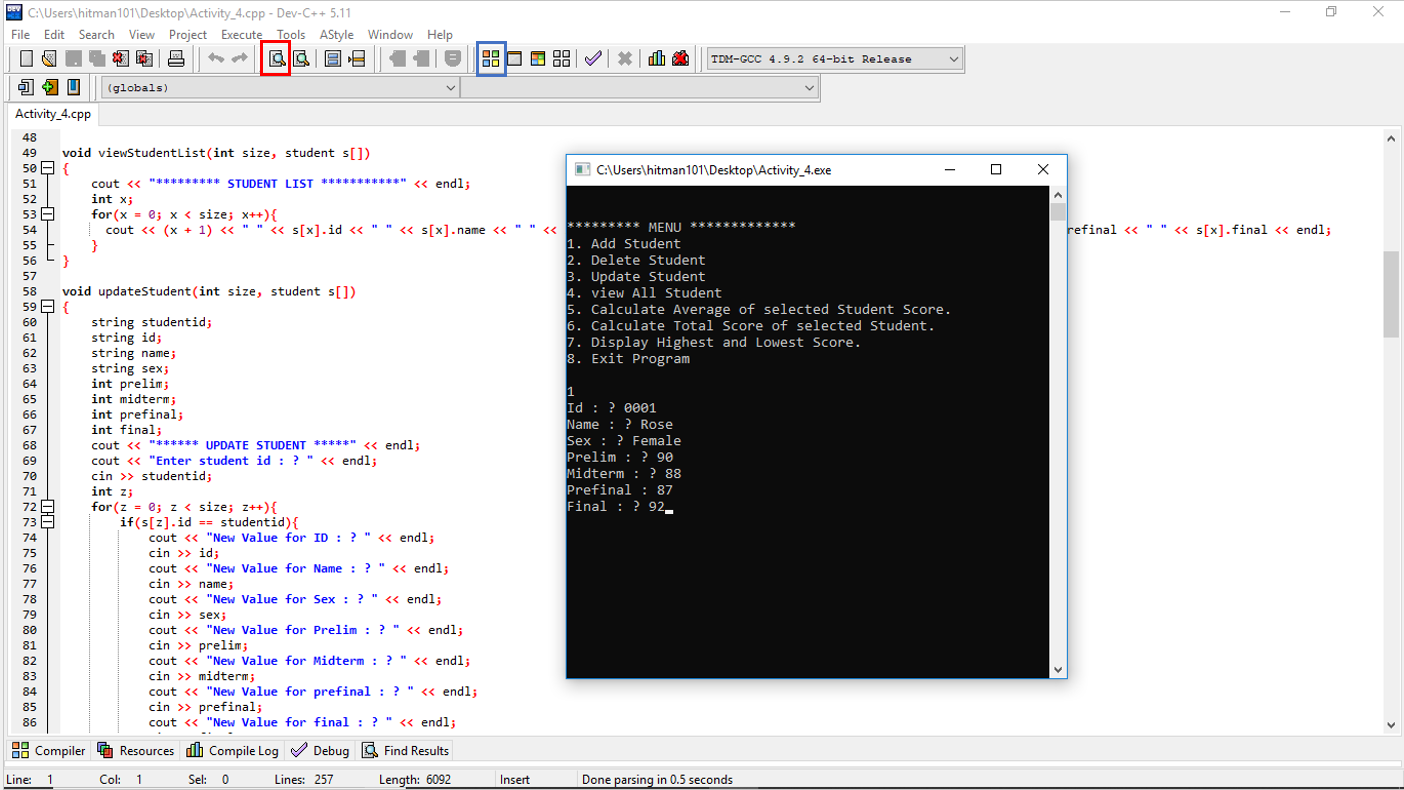
\includegraphics[width=\textwidth]{fig/example.png}
	\caption{Your beaultiful example picture}
	\label{fig:example}
\end{figure*}
\subsection{Why the Technical Problem Is Important}
The technical problem is important because \blank{}. Failing to address the problem well cause \blank{}. \explain{Here is an example.} For example, in Figure~\ref{fig:example}, the technical problem is critical to \blank{solve the constraints in the red box, so the requirement is not satisfied because of A}.

\subsection{Why the Technical Problem Is Challenging}
The technical problem \blank{} is challenging because of \blank{term 1}, \blank{term 2}, and \blank{term 3}. \explain{Here is an example.} \blank{Term 1} is challenging because \blank{}. For example, in Figure~\ref{fig:example}, \blank{term 1} introduces challenges in \blank{solving the constraints in the blue box}. Unfortunately, addressing \blank{term 1} is \blank{an NP-hard problem}. Existing techniques \blank{can only provide an approximate,}which is not sufficient to address the technical problem because \blank{}.   

\subsection{Our Insights}
Our strategy is based on \blank{} insights, which are \blank{},\blank{}, and \blank{}. \explain{Here is an example} For \blank{insight 1}, it is valid because \blank{}. For example, in Figure~\ref{fig:example}, \blank{the code in lines 81 - 88} they meet the \blank{insght 1} becuase \blank{}.  

\subsection{Core Idea}
The core idea of our strategy consists of \blank{} steps. \explain{Here is an example.} First, based on \blank{insight 1}, it does \blank{}. For example, in Figure~\ref{fig:example}, our strategy first \blank{identifies the code that meets requirement A, such as the code in lines 85-87}. This step is good because \blank{}. Second, based on \blank{insight 2}, it does \blank{}. For example, in Figure~\ref{fig:example}, our strategy does \blank{}. This step is good because \blank{}.


\section{Theat Model and Assumptions}
\explain{This is for security papers only. please check~\cite{threatmodel}. Here is an example}
We follow the same threat model used in previous work~\cite{}. Specifically, we assume the OS/hardware is uncompromised. We do not consider side-channel attacks. 
\section{Approach Overview}
\eat{总分结构}
We realize our strategy as a framework/tool, \toolname, of which workflow is shown in Figure~\ref{fig:workflow}. The input of \toolname is \blank{}. The output of \toolname is \blank{}. \toolname has \blank{} components/steps. The first component is \blank{}, which accepts \blank{} and outputs \blank{}. Intuitively, the first component does \blank{}. We do this because \blank{}. The second component is \blank{}, which accepts \blank{} and outputs \blank{}. Intuitively, the second component does \blank{}. We do this because \blank{}. The third component is \blank{}, which accepts \blank{} and outputs \blank{}. Intuitively, the third component does \blank{}. We do this because \blank{}. 

\begin{figure*}[t!]
    \centering
    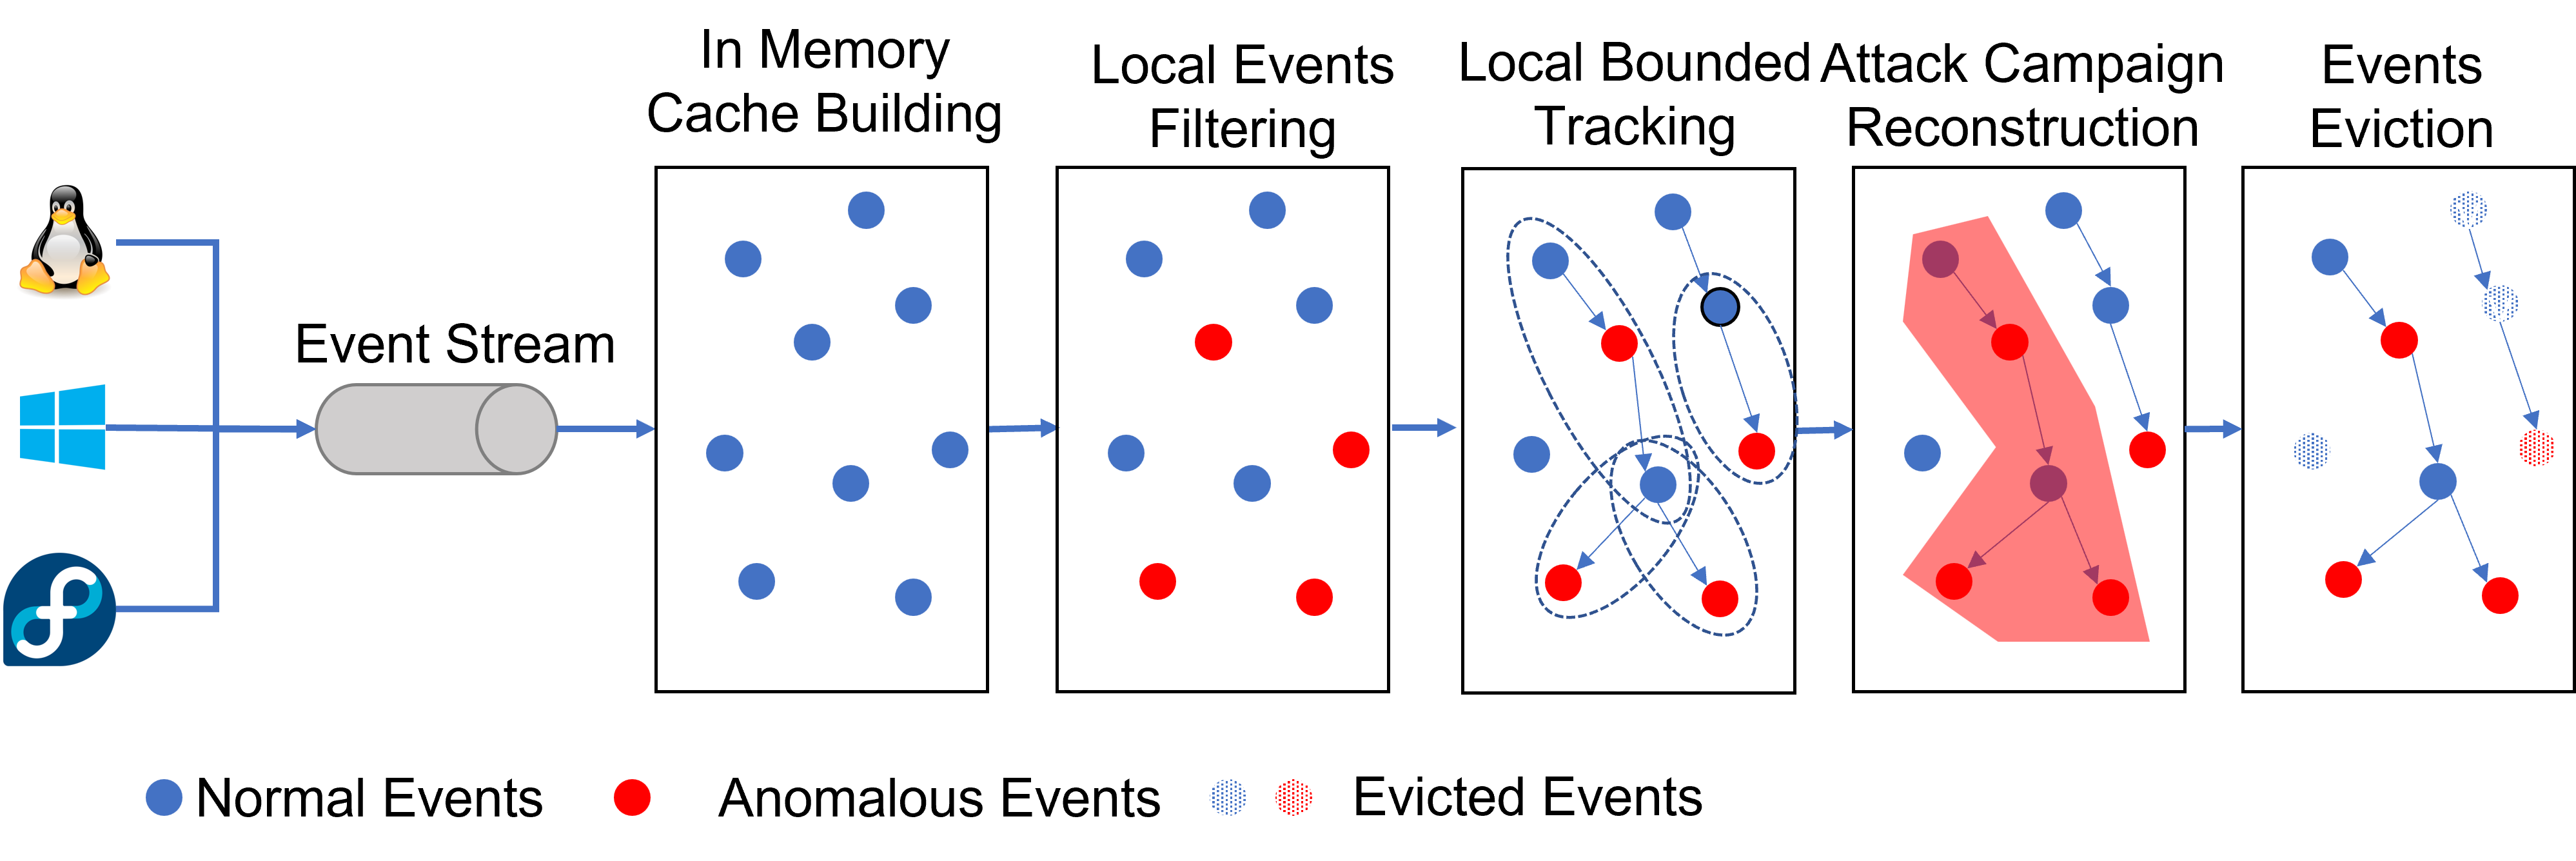
\includegraphics[width=\textwidth]{fig/workflow.png}
	\caption{Your beaultiful workflow picture}
	\label{fig:workflow}
\end{figure*}
\section{Design}
In this section, we discuss the design details of the components of \toolname. 
\explain{I will make an example for one component, add more based on your need}
\subsection{Component 1}
The goal of \blank{the name of component 1} is \blank{}. We use  \blank{the name of component 1} because \blank{}. 

On the high-level, \blank{the name of component 1} is a \blank{a few sentences for high level description}. We need to address \blank{} engineering problems in component \blank{}, which are \blank{}, \blank{}, and \blank{}. 

\explain{There are some examples}
To address the engineering/technical problem \blank{}, we leverage a data structure \blank{}. This data structure is a graph whose nodes are \blank{} and edges are \blank{}. This graph is an attributed graph. Therefore, each node has an attribute that represents \blank{}. Formally, we define the graph as \blank{your mathematical equations}.

To address the engineering/technical problem \blank{}, we leverage a deep learning model \blank{}. We choose this deep learning model \blank{} because it can \blank{}. The deep learning model consists of \blank{} components, which are \blank{}. Formally, the deep learning model is \blank{your math}.We choose this deep learning model \blank{} because it can \blank{}. The deep learning model consists of \blank{} components, which are \blank{}. Formally, the deep learning model is \blank{your math}.



To address the engineering/technical problem \blank{}, we propose a heuristic algorithm. On the high level, our algorithm does \blank{}. The formal pseudocode is in Algorithm~\ref{}. Specifically, \blank{discuss the critical steps in the Algorithm}




\section{Evaluation}\label{section5}
To evaluate \toolname, we focus on answering following research questions



\textbf{RQ 1}: Does \toolname improve the aspect \blank{} for the technical requirement? \explain{Add more if you have more than one aspects}

%Process based Precision,recall,F1,alarm rate

\textbf{RQ 2}: Does \toolname address the technical problem?

\textbf{RQ 3}: Do the insights valid emprically?


\textbf{RQ 4}: Is \toolname useful in read production environment? \explain{optional, if you are lucky, you will have this}.

\subsection{Experiment Environment and Datasets}
The hardware platform of our experiment environment is \blank{}. The OS is \blank{}. The software environment is \blank{}. 

We use \blank{} datasets because \blank{}. 

We use \blank{} as baselines because \blank{}


\subsection{RQ 1: Better Satisfy the Requirement in Aspect 1}
We evaluate whether \toolname better satisfies the aspect \blank{} of the technical requirement by measuring the metric \blank{}. We use this metric because \blank{many other papers use it or other solid reasons. }  To measure the metric  \blank{}, we do \blank{}. Our measurement is solid because \blank{}. \explain{sometimes the reasons for solid are obvious, then you may omit the discisson}.

We report the result in Table/Figure X. Particularly, \toolname is XX\% better than the baselines. This result proves that \toolname can better satisfy the requirement. 


\subsection{RQ 2: Does \toolname Address the Technical Problem}
We evaluate whether \toolname address the technical problem \blank{} by measuring the metric \blank{}. We use this metric because \blank{many other papers use it or other solid reasons. }  To measure the metric  \blank{}, we do \blank{}. Our measurement is solid because \blank{}. \explain{sometimes the reasons for solid are obvious, then you may omit the discisson}.

We report the result in Table/Figure X. Particularly, \blank{}. This result proves that \toolname address the technical problem.

\subsection{RQ 3: Do the Insights Valid}
We evaluate whether the insights are valud by measuring the metrics \blank{}. We use this metric because \blank{many other papers use it or other solid reasons. }  To measure the metric  \blank{}, we do \blank{}. Our measurement is solid because \blank{}. \explain{sometimes the reasons for solid are obvious, then you may omit the discisson}.

We report the result in Table/Figure X. Particularly, \blank{}. This result proves that \toolname address the technical problem.

\section{Threats to Validity}
\explain{This is for SE papers only. Discuss potential threats to your evaluation protocal that may lead to biased measurement and how you address these threats. see:https://mydissertationeditor.com/threats-to-validity/}



\section{Related Work}


\section{Discussion}
\explain{This section is for Security papers only. Discuss the limitation of your approach. Note that you should be careful here. You should avoid discussing very lithal bugs in your design. Focus on the open problems or issues related to your threat model and assumption. Below is an example. }
Our approach assumes that \blank{}. Although this is a practical assumption and used by many academic and industrial solutions, attackers may compromise the assumption by \blank. Although it is important to address the possible attacks out of the assumption of this paper, they are beyond the scope of this paper.
\section{Conclusion}
% \section{Acknowledgments}

%for ACM papers
\bibliographystyle{ACM-Reference-Format}
%for IEEE papers
%\bibliographystyle{IEEEtran} %for IEEE papers
\bibliography{references}


\end{document}
